\section{Measurement Model}
We consider the problem of recovery of a signal from its modulo measurements obtained through compressive sensing. Simply put, we aim to recover $\mathbf{x^*}\in \R^n$ from the modulo measurements $y_i=\mod(\langle \mathbf{a_i} \cdot \mathbf{x^*} \rangle,R)$ for $i = \{1,2,...,m\}$, where $\mod$ is modulo operation with respect to $R$. Typically, $m<n$. For simplicity, we assume that the modulo function operates only within two periods, one on the either side of the origin, as shown in the Fig.~\ref{fig:graph}. We construct $\mathbf{A} = \left[\mathbf{a_1~a_2~...~a_m}\right]^T$ with i.i.d. Gaussian entries. The primary assumption in our model is that the natural signal $\mathbf{x^*}$ is $s-$sparse in a chosen basis. 

\begin{figure}[h]
	\begin{center}
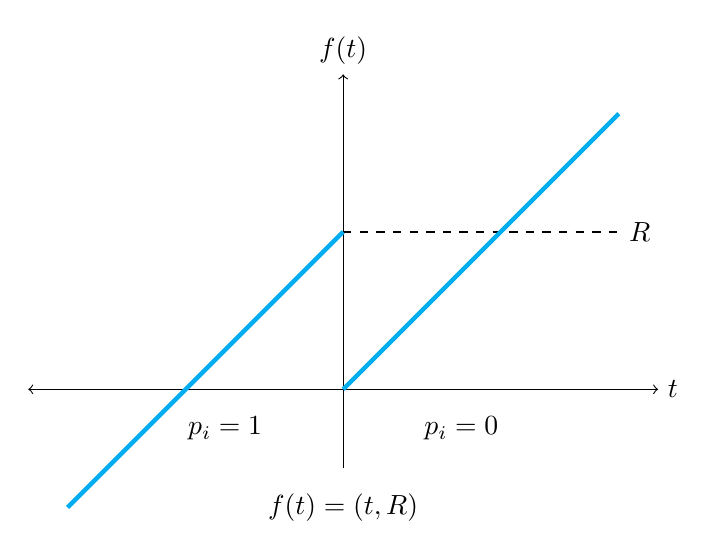
\begin{tikzpicture}
\draw[<->] (-4,0) -- (4,0) node[right] {$t$};
\draw[->] (0,-1) -- (0,4) node[above] {$f(t)$};
\draw[scale=0.5, dashed, thick] (0,4)--(7,4) node[right]{$R$};
\draw (1.5,-0.5) node(below) {$p_i = 0$};
\draw (-1.5,-0.5) node(below) {$p_i = 1$};
\draw (0,-1.5) node(right) {$f(t) = \mod(t,R)$};
\draw[scale=0.5,domain=-7:0,smooth,variable=\x,cyan, ultra thick] plot ({\x},{\x+4});
\draw[scale=0.5,domain=0:7,smooth,variable=\x,cyan, ultra thick]  plot ({\x},{\x});
\end{tikzpicture}
\end{center}
\caption{\emph{Modified modulo function for the given problem}}
\label{fig:graph}
\end{figure}

We can write the modified equation for the modulo operation under consideration as:
$$
f(t) = \mod(t,R) = t+\left( \frac{1-\sgn(t)}{2}\right)R,
$$
where $\sgn(t)$ is a signum function.

For the measurement model of the given problem, 
We define the corrected linear measurements as: 

$$
y_{c,i} =\langle \mathbf{a_i} \cdot \mathbf{x^*} \rangle.
$$

We also define the bin-index $p^*_i$ as,
$$
p^*_i = \frac{1-\sgn(\langle \mathbf{a_i} \cdot \mathbf{x^*} \rangle)}{2}.
$$
Thus,
$$
y_i = \langle \mathbf{a_i} \cdot \mathbf{x^*} \rangle + p^*_iR = y_{c,i}+p^*_iR.
$$

It is evident that if we can recover $\mathbf{p^*}$ successfully, we can calculate the correct compressed measurements $\langle \mathbf{a_i} \cdot \mathbf{x^*} \rangle$ and use them to reconstruct $\mathbf{x^*}$ with any sparse recovery algorithm such as CoSaMP.


\section{Reconstruction Algorithm}

In this section, we describe our AltMin based approach to recover $\mathbf{x^*}$ and $\mathbf{p^*}$, given $\mathbf{y, A}, s, R$. We call our algorithm MoRAM - Modulo Reconstruction using Alternative Minimization. Our approach comprises of two steps: (i) estimate initialization step, and (ii) Descent step through alternative minimization.

\subsection{Initialization: Method 1: MoRAM}
\label{sec:init}
Similar to many non-convex techniques, MoRAM also requires an initial estimate $\mathbf{{x}^0}$ that is close to the true signal $\mathbf{{x}^*}$. The basic idea is to calculate the significant indices (or the support of $\mathbf{{x}^*}$, $S=support(\mathbf{{x}^*})$) using the suitable biased estimators, and then calculate the initial estimate using a first order biased estimator $M$ only for those significant indices contained in the support of $\mathbf{{x}^*}$. This initialization procedure is quite simple, and requires the tuning of only one parameter, the sparsity ($s$).

For support estimation, we use measurements $y_{i}$ to construct a biased estimator $L$, for which the marginal $L_{jj}$ corresponding to the $j^{th}$ element is given by:
$$
L_{jj} = \frac{1}{m}\sum_{i=1}^{m}y_{i}^2 a_{ij}^2,~~~\textnormal{for}~~~~j \in {1,...,n}.
$$
Note that the expectation $\mathbb{E}[\mathbf{L}]$ is given by,
$$
\mathbb{E}[L_{jj}] = 4x_{j}^{*2}+2R^2(1-c_1)-2R\norm{\mathbf{{x}^*}}c_2~~~~~\textnormal{where,}~c_1,c_2 \in \mathbb{R}
$$
indicating that a clear separation exists for values of expectation for $j \in S$ and $j \in S^c$, because $x_j$ is zero for $j \in S^c$ and non-zero otherwise. Therefore, we can form the approximation of the support, $\widehat{S}$ by collecting the indices of the higher magnitude elements of $\mathbb{E}[L]$. With the support known, we can throw away the columns of $\mathbf{A}$ corresponding to $j \in S^c$ for the next steps. This would make the computation faster.

Next step is to obtain the initial estimate using the first order estimator $\mathbf{M}$, defined as:
$$
M_{jj} = \frac{1}{m}\sum_{i=1}^{m}y_{i}a_{ij},~~~\textnormal{for}~~~~j \in S.
$$
To calculate $\mathbf{{x}^0}$, we use the fact that
$$
\mathbb{E}[\mathbf{M}] = \left( 1 - \sqrt{\frac{2}{\pi}}\frac{R}{2} \right) \mathbf{{x}^*}.
$$
Given enough number of samples, the sample mean of the above estimator lie very close to the expectation value. Thus, we can calculate the initial estimate $\mathbf{{x}^0}$ as:
\begin{equation}
	\mathbf{{x}^0_j} = 
	\begin{cases}
	\frac{1}{m}\sum_{i=1, j \in S}^{m}y_{i}a_{ij}~~~,& \text{if } j \in S \\
	0,              & j \in S^c.
	\end{cases}
	\label{eq:init}
\end{equation}
However, it should be noted that the quality of the initial estimate is a direct function of the number of measurements $(m)$. 


\begin{algorithm}[H]
	\caption{\textsc{MoRAM}}
	\label{alg:DMF}
	\begin{algorithmic}
		\State\textbf{Inputs:} $\mathbf{y}$, $\mathbf{A}$, $s$, $R$
		\State\textbf{Output:}  $\widehat{x}$
		\State $m,n \leftarrow \mathrm{size}(\mathbf{A})$ 
		\State $s_p \leftarrow 0.1\cdot m$
		\State \textbf{Initialization}
		\State $\mathbf{x^0} \leftarrow \textrm{Oracle}(\mathbf{y, A})$ 
		\State \textbf{Alternative Minimization}
		\For {$l =0:\mathrm{N}$}
		\State $\mathbf{{p}^{t}} \leftarrow \frac{\mathbf{1}-\sgn(\langle \mathbf{A} \cdot \mathbf{x^t} \rangle)}{2}$
		\State $\mathbf{{x}^{t+1}}\leftarrow \argmin_{[\mathbf{x~d}]^T \in \mathcal{M}_{s+s_p}}\norm{\begin{bmatrix} \mathbf{A} & \mathbf{I} \end{bmatrix} \begin{bmatrix} \mathbf{x} \\ \mathbf{d} \end{bmatrix} - \mathbf{y}}_2^2 = \cosamp(\frac{1}{\sqrt{m}}\begin{bmatrix} \mathbf{A} & \mathbf{I} \end{bmatrix},\frac{1}{\sqrt{m}}\mathbf{y},s+s_p,[\mathbf{x^t~~p^t}]^T)$
		\EndFor
	\end{algorithmic}
\end{algorithm}

\subsection{Initialization: Method 2: Re-Calculated Measurements (RCM)}
The initial estimate we get with MoRAM usually has a relative error in the ranges of 1 to 1.5 depending on number of measurements. As we can see in the Fig.~\ref{fig:graph}, such initial estimates are not good enough for accurate recovery of the signal using robust CoSaMP algorithm. In general, with the decreasing value of the signal strength (or, with the increasing value of $R$), the error in reconstruction using robust CoSaMP increases. This is also evident in the results shown in the table~\ref{Tab2}. To overcome this issue, we propose a method to re-calculate the measurements which is effective in the cases where signal strengths are low compared to the value of $R$, but can also be used for the other case. To understand the reasoning behind it, we will first try to understand the effect of modulo operation on the linear measurements.

\subsubsection{Effect of Modulo Operation} 
We observe the histograms of the $\mathbf{Ax^*}$(Fig.~\ref{fig:hist1}) and $\mathbf{\mod(\mathbf{Ax^*})}$(Fig.~\ref{fig:hist2}) to understand the information we can obtain from the modulo measurements. We are particularly interested in the case where signal strengths are low compared to the value of $R$, nevertheless, we also analyze the other case when $R$ is less than the signal strength. Here, we define $\rho$ as maximum element in $\mathbf{Ax^*}$. $\rho$ is bounded by a real number with very high probability, as the distribution of $\mathbf{Ax^*}$ is Gaussian.
In Fig.~\ref{fig:hist2} and Fig.~\ref{fig:hist3}, we can see the histogram after the modulo operation for both the cases: $R>\rho$ and $R<\rho$. Comparing these histograms with the histogram of true measurements (Fig.~\ref{fig:hist1}), we can observe how the values of first histogram translates into second or third when the modulo operation is applied. We can draw following conclusions:
\begin{itemize}
	\item Only the values lying on the negative side of the x-axis are going to be affected.
	\item Values lying very close to the origin on the negative side of the x-axis in the first histogram, would now shift by $R$, and would occupy a place very close to $R$ in second histogram. For $R>\rho$, this region is shaded with green color in Fig.~\ref{fig:hist2}. Correct bin-value for the elements in $\mathbf{y}$ with value lying between $\rho$ and $R$ is $p_{rcm,i} = 1$.
	\item For $R>\rho$, histogram of the positive region very close to the origin would remain unaffected. This region is shaded with orange color in Fig.~\ref{fig:hist2}. Correct bin-value for all the elements in $\mathbf{y}$ with value lying between $0$ and $R-\rho$ is $p_{rcm,i} = 0$.
	\item Nothing can be concluded for measurements lying in between the above mentioned ranges. This region is shaded with gray color in Fig.~\ref{fig:hist2} and Fig.~\ref{fig:hist3}. Correct bin-value cannot be identified for this region, so we assign all the elements in $\mathbf{y}$ with value lying between $0$ and $(R-\rho)$ as $p_{rcm,i} = 0$. The lower and upper bounds ($t_l \& t_u$) of this disputed region can be obtained as, 
	$$t_l = \max(0, R-\rho)$$
	$$t_u = \max(\rho, R)$$.
	\item Irrespective of relationship between $\rho$ and $R$, all the values lying in the negative half of the real line have the bin-value equal to $1$, and all the values greater than $R$ have the bin-value equal to $0$.
\end{itemize}
We divide the number line in the following 5 intervals, and assign the bin-value accordingly:
\begin{equation}
\mathbf{{p}_{rcm,i}} = 
\begin{cases}
1,& \text{if } \mathbf{y_i} <0 \\
0,& \text{if } 0\leq \mathbf{y_i} < t_l \\
0,& \text{if } t_l\leq \mathbf{y_i} < t_u \\
1,& \text{if } t_u \leq \mathbf{y_i} < R \\
0,& \text{if } R  \leq \mathbf{y_i}. \\
\end{cases}
\label{eq:rcm}
\end{equation}
Thus, we can identify the correct bin values for part of the measurements just by observing their magnitude. Number of elements for which we can identify the bin-values correctly depends on the difference between $\rho$ and $R$.
\begin{figure}[h]
	\begin{center}
		\begin{tikzpicture}
		\def\normaltwo{\x,{3*1/exp(((\x)^2)/2)}}
		\def\y{4.4}
		
		%\fill [fill=orange!60] (2.6,0) -- plot[domain=0:4.4] (\normaltwo) -- ({\y},0) -- cycle;
		
		% Draw and label normal distribution function
		\draw[color=blue,domain=-3:3,thick] plot (\normaltwo) node[right] {};
		\draw[<->] (-5,0) -- (5,0) node[right] {$\mathbf{Ax^*}$};
		\draw[<->] (0,-1) -- (0,4);

		\draw (-3,-0.5) node(below) {$-\rho$};
		\draw (-4,-0.5) node(below) {$-R$};
		\draw (3,-0.5) node(below) {$\rho$};
		\draw (4,-0.5) node(below) {$R$};
		
		\foreach \x in {-3,-4,3,4}
		{        
			\coordinate (A\x) at ($(0,0)+(\x*1cm,0)$) {};
			\draw ($(A\x)+(0,5pt)$) -- ($(A\x)-(0,5pt)$);

		}
%		\draw (-1.5,-0.5) node(below) {$p_i = 1$};
%		\draw (0,-1.5) node(right) {$f(t) = \mod(t,R)$};
%		\draw[scale=0.5,domain=-7:0,smooth,variable=\x,cyan, ultra thick] plot ({\x},{\x+4});
%		\draw[scale=0.5,domain=0:7,smooth,variable=\x,cyan, ultra thick]  plot ({\x},{\x});
		\end{tikzpicture}
	\end{center}
	\caption{\emph{Histogram of $\mathbf{Ax^*}$}}
	\label{fig:hist1}
\end{figure}
\begin{figure}[h]
	\begin{center}
		\begin{tikzpicture}
		\def\normaltwo{\x,{3*1/exp(((\x)^2)/2)}}
		\def\normalone{\x,{3*1/exp(((\x-4)^2)/2)}}
		\def\normalsum{\x,{3*1/exp(((\x-4)^2)/2)+3*1/exp(((\x)^2)/2)}}
		\def\y{3}
		\def\fy{3*1/exp(((\y-4)^2)/2)}
		\fill [fill=orange!60] (0,0) -- plot[domain=0:1] (\normaltwo) -- (1,0) -- cycle;
		\fill [fill=green!60] (3,0) -- plot[domain=3:4] (\normalone) -- (4,0) -- cycle;
		\fill [fill=gray!30] (1,0) -- plot[domain=1:3] (\normalsum) -- (3,0) -- cycle;
		% Draw and label normal distribution function
		\draw[color=blue,domain=-0:3,dashed,thick] plot (\normaltwo) node[right] {};
		\draw[color=blue,domain=1:4,dashed,thick] plot (\normalone) node[right] {};
		\draw[color=blue,domain=-0:4,thick] plot (\normalsum) node[right] {};
		\draw[<->] (-5,0) -- (5,0) node[right] {$\mathbf{Ax^*}$};
		\draw[<->] (0,-1) -- (0,4);
		\draw[dashed] ({\y},{\fy}) -- ({\y},0);
		\draw[dashed] ({4},{3}) -- ({4},0);
		\draw[dashed] ({1},{\fy}) -- ({1},0);
		\draw (-3,-0.5) node(below) {$-\rho$};
		\draw (-4,-0.5) node(below) {$-R$};
		\draw (3,-0.5) node(below) {$\rho$};
		\draw (4,-0.5) node(below) {$R$};
		\draw (1,-0.5) node(below) {$R-\rho$};
		\draw (0.5,1) node(below) {$p_i=0$};
		\draw (3.5,1) node(below) {$p_i=1$};
		\draw (2,0.5) node(below) {$p_i=0$};
		\foreach \x in {-3,-4,1,3,4}
		{        
			\coordinate (A\x) at ($(0,0)+(\x*1cm,0)$) {};
			\draw ($(A\x)+(0,5pt)$) -- ($(A\x)-(0,5pt)$);
			
		}
		%		\draw (-1.5,-0.5) node(below) {$p_i = 1$};
		%		\draw (0,-1.5) node(right) {$f(t) = \mod(t,R)$};
		%		\draw[scale=0.5,domain=-7:0,smooth,variable=\x,cyan, ultra thick] plot ({\x},{\x+4});
		%		\draw[scale=0.5,domain=0:7,smooth,variable=\x,cyan, ultra thick]  plot ({\x},{\x});
		\end{tikzpicture}
	\end{center}
	\caption{\emph{Histogram of $\mod(\mathbf{Ax^*})$, $R>\rho$}}
	\label{fig:hist2}
\end{figure}

\begin{figure}[!h]
	\begin{center}
		\begin{tikzpicture}
		\def\normaltwo{\x,{3*1/exp(((\x)^2)/2)}}
		\def\normalone{\x,{3*1/exp(((\x-2)^2)/2)}}
		\def\normalsum{\x,{3*1/exp(((\x-2)^2)/2)+3*1/exp(((\x)^2)/2)}}
		\def\y{3}
		\def\fy{3*1/exp(((\y-4)^2)/2)}
		\fill [fill=orange!60] (-1,0) -- plot[domain=-1:0] (\normalone) -- (0,0) -- cycle;
		\fill [fill=green!60] (2,0) -- plot[domain=2:3] (\normaltwo) -- (3,0) -- cycle;
		\fill [fill=gray!30] (0,0) -- plot[domain=0:2] (\normalsum) -- (2,0) -- cycle;
		% Draw and label normal distribution function
		\draw[color=blue,domain=-0:3,dashed,thick] plot (\normaltwo) node[right] {};
		\draw[color=blue,domain=-1:2,dashed,thick] plot (\normalone) node[right] {};
		\draw[color=blue,domain=-0:2,thick] plot (\normalsum) node[right] {};
		\draw[<->] (-5,0) -- (5,0) node[right] {$\mathbf{Ax^*}$};
		\draw[<->] (0,-1) -- (0,4);
		%\draw[dashed] ({\y},{\fy}) -- ({\y},0);
		\draw[dashed] ({-1},{2}) -- ({-1},0);
		\draw[dashed] ({3},{2}) -- ({3},0);
		%\draw[dashed] ({1},{\fy}) -- ({1},0);
		\draw (-3,-0.5) node(below) {$-\rho$};
		\draw (-2,-0.5) node(below) {$-R$};
		\draw (3,-0.5) node(below) {$\rho$};
		\draw (2,-0.5) node(below) {$R$};
		\draw (-1,-0.5) node(below) {$-\rho+R$};
		\draw (-0.5,1) node(below) {$p_i=0$};
		\draw (2.5,1) node(below) {$p_i=1$};
		\draw (1,0.5) node(below) {$p_i=0$};
		\foreach \x in {-3,-2,-1,3,2}
		{        
			\coordinate (A\x) at ($(0,0)+(\x*1cm,0)$) {};
			\draw ($(A\x)+(0,5pt)$) -- ($(A\x)-(0,5pt)$);
			
		}
		%		\draw (-1.5,-0.5) node(below) {$p_i = 1$};
		%		\draw (0,-1.5) node(right) {$f(t) = \mod(t,R)$};
		%		\draw[scale=0.5,domain=-7:0,smooth,variable=\x,cyan, ultra thick] plot ({\x},{\x+4});
		%		\draw[scale=0.5,domain=0:7,smooth,variable=\x,cyan, ultra thick]  plot ({\x},{\x});
		\end{tikzpicture}
	\end{center}
	\caption{\emph{Histogram of $\mod(\mathbf{Ax^*})$, $R<\rho$}}
	\label{fig:hist3}
\end{figure}

Once we identify the correct bin-values for part of the measurements, we can re-calculate corrected measurements as,
$$
\mathbf{y_{rcm} = y + p_{rcm}R}.
$$
We use this corrected measurements $\mathbf{y_{rcm}}$ to calculate the initial estimate $\mathbf{{x}^0}$ using the MoRAM algorithm described in sec.~\ref{sec:init}. Because of correctness of partial number of measurements, the initial estimate obtained in this case better than one obtained only through MoRAM as depicted in Fig.~\ref{fig:init_comp}.

 \begin{figure}[t]
 	\begin{center}
 		%\vspace{-0em}
 		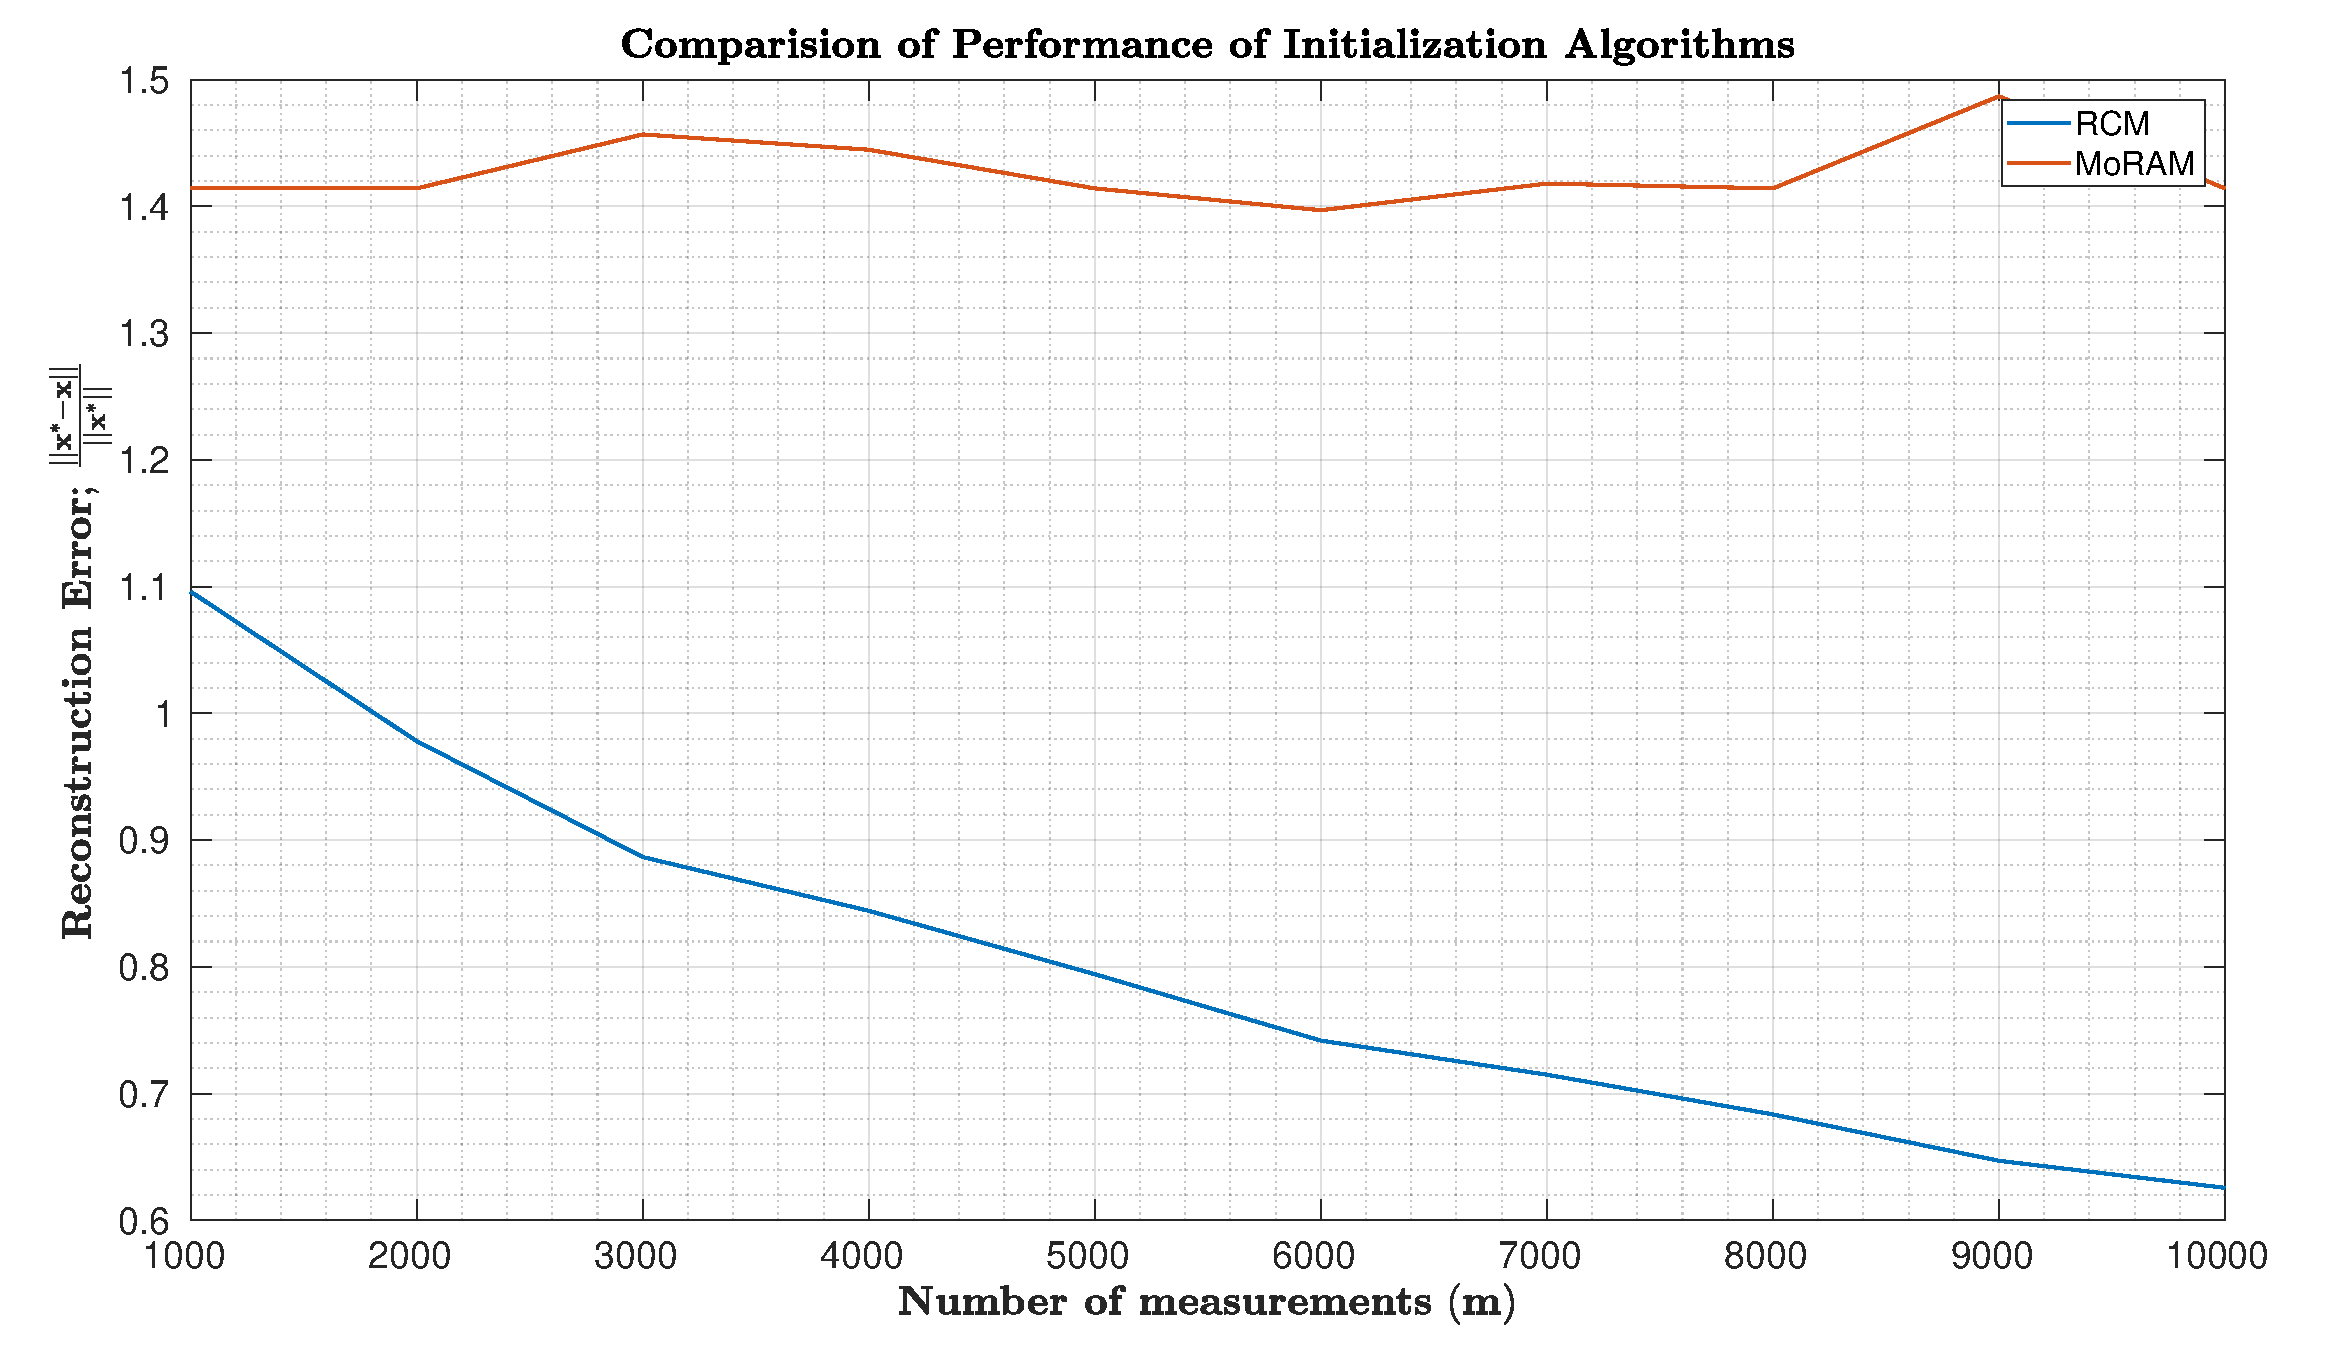
\includegraphics[width=\linewidth]{./fig/MoRAM_RCM_compare.pdf}
 	\end{center}
 	\caption{}
 	\label{fig:init_comp}
 \end{figure}

\subsection{Alternative Minimization}
\label{sec:altmin}

Using Eq.~\ref{eq:init}, we calculate the initial estimate of the signal $\mathbf{{x}^0}$ which is relatively close to the true vector $\mathbf{x^*}$. Starting with $\mathbf{{x}^0}$, we  calculate the estimates $\mathbf{p}$ and $\mathbf{x}$ in alternating fashion to converge to the original signal $\mathbf{x^*}$. At each iteration of our Alternative Minimization, we use the current estimate of the signal ${\mathbf{x^t}}$ to get the value of the bin-index vector $\mathbf{{p}^t}$ as following:
\begin{equation}
\mathbf{{p}^{t}} = \frac{\mathbf{1}-\sgn(\langle \mathbf{A} \cdot \mathbf{x^t} \rangle)}{2}.
\label{step1}
\end{equation}

 
 Given $\mathbf{x^0}$ is close to $\mathbf{x^*}$, $\mathbf{p^0}$ would also be close to $\mathbf{p^*}$. Ideal way is to calculate the correct compressed measurements $\mathbf{y^t_c}$ using $\mathbf{p^t}$, and use $\mathbf{y_c}$ with CoSaMP to calculate the next estimate $\mathbf{{x}_{t+1}}$. Thus,


$$
\mathbf{y^t_c} = \langle \mathbf{A}\mathbf{x_{t}} \rangle = \mathbf{y} - \mathbf{p^t}R,
$$
$$
\mathbf{{x}^{t+1}} = \argmin_{\mathbf{x} \in \mathcal{M}_s}\norm{\mathbf{Ax} - \mathbf{y^t_c}}_2^2, %~~\mathrm{s.to}~~x^* \in \mathcal{M}_s,
$$

\begin{equation}
\implies \mathbf{{x}^{t+1}} = \cosamp(\frac{1}{\sqrt{m}}\mathbf{A},\frac{1}{\sqrt{m}}\mathbf{y^t_c},s,\mathbf{x_t}).
\label{eq:cosamp}
\end{equation}


 However, it should be noted that even the small error $\mathbf{d} = \mathbf{p^t - p^*}$ would reflect heavily in the calculation of $\mathbf{y^t_c}$, as each incorrect bin-index would add a noise of the magnitude $R$ in $\mathbf{y^t_c}$. Experiments suggest that the CoSaMP is not robust enough to cope up with such large errors in $\mathbf{y^t_c}$. To tackle this issue, we augmented the sparse recovery problem using the fact that the nature of error $\mathbf{d^t_p}$ is sparse; and each erroneous element of $\mathbf{p}$ adds a noise of the magnitude $R$ in $\mathbf{y^t_c}$. We take the sparsity of $\mathbf{d^t}$ to be $s_p = 0.1\times m$, suggesting that at most the $10\%$ of the total elements are classified with wrong bin-indices.
 
 The augmented optimization problem becomes,
  
$$
\mathbf{{x}^{t+1}}=\argmin_{[\mathbf{x~d}]^T \in \mathcal{M}_{s+s_p}}\norm{\begin{bmatrix} \mathbf{A} & \mathbf{I} \end{bmatrix} \begin{bmatrix} \mathbf{x} \\ \mathbf{d} \end{bmatrix} - \mathbf{y}}_2^2, %~~\mathrm{s.to}~~x^* \in \mathcal{M}_s,
$$
\begin{equation}
\implies \mathbf{{x^{t+1}}} = \cosamp(\frac{1}{\sqrt{m}}\begin{bmatrix} \mathbf{A} & \mathbf{I} \end{bmatrix},\frac{1}{\sqrt{m}}\mathbf{y},s+s_p,[\mathbf{x^t~~p^t}]^T).
\label{eq:robcosamp}
\end{equation}
We call the step in Eq.~\ref{eq:robcosamp} a Robust CoSaMP. 
However, for using CoSaMP , it is required to specify the total sparsity value $(s +s_p)$, where $s_p$ is unknown. Thus, we employ Basis pursuit instead of CoSaMP, which doesn't rely on sparsity. The robust formulation of basis pursuit is referred as Justice Pursuit (JP) in the literature, specified in Eq.~\ref{eq:jp}.
\begin{equation}
\implies \mathbf{{x^{t+1}}} = JP(\frac{1}{\sqrt{m}}\begin{bmatrix} \mathbf{A} & \mathbf{I} \end{bmatrix},\frac{1}{\sqrt{m}}\mathbf{y},[\mathbf{x^t~~p^t}]^T).
\label{eq:jp}
\end{equation}
We repeat the steps of bin index calculation (as in Eq.~\ref{step1}) and sparse recovery (as in Eq.~\ref{eq:cosamp} or Eq.~\ref{eq:robcosamp} or Eq.~\ref{eq:jp}) alternatively for $\mathrm{N}$ iterations. While the sparse recovery with robust CoSaMP (Eq.~\ref{eq:robcosamp}) improves the reconstruction performance for large values of $R$ by making the sparse recovery step less susceptible to the errors, CoSaMP can also used in its original form (as in Eq.~\ref{eq:cosamp}) for lower values of $R$. Nevertheless, the best performing recovery algorithm uses Justice Pursuit, which is able to produce perfectly converging results, as described in experimental section.

Thus, we can have two variants of the MoRAM algorithm: (i)MoRAM with CoSaMP, (ii) MoRAM with robust CoSaMP, and (iii) MoRAM with Justice Pursuit. 

%$$
%\norm{\begin{bmatrix} \mathbf{A} & \mathbf{I} \end{bmatrix} \begin{bmatrix} \mathbf{x^*} \\ \mathbf{d} \end{bmatrix} - \mathbf{y}}_2^2.
%$$

%


\subsection{Experiments}

\subsubsection{Analyzing sensitivity towards the initial estimate}
For this experiment, we use a synthetic signal generated randomly with $n=1000$ and $s=20$. 
Our aim is to analyze the sensitivity of our algorithm towards the initial estimate $\mathbf{x^0}$. %Currently, in the absence of a suitable initialization method, 
For that, we compute the initial estimate $\mathbf{x^0}$ by adding a Gaussian noise to the original signal. In Fig.~\ref{fig:pl}, we plot the variation of the relative reconstruction error ($\frac{\norm{\mathbf{x^*-x^N}}}{\norm{\mathbf{x^*}}}$) with the relative error in initial estimate ($\frac{\norm{\mathbf{x^*-x^0}}}{\norm{\mathbf{x^*}}}$). We plot the similar curves for different values of number of measurements $m$.
\begin{figure}[t]
	\begin{center}
		%\vspace{-0em}
		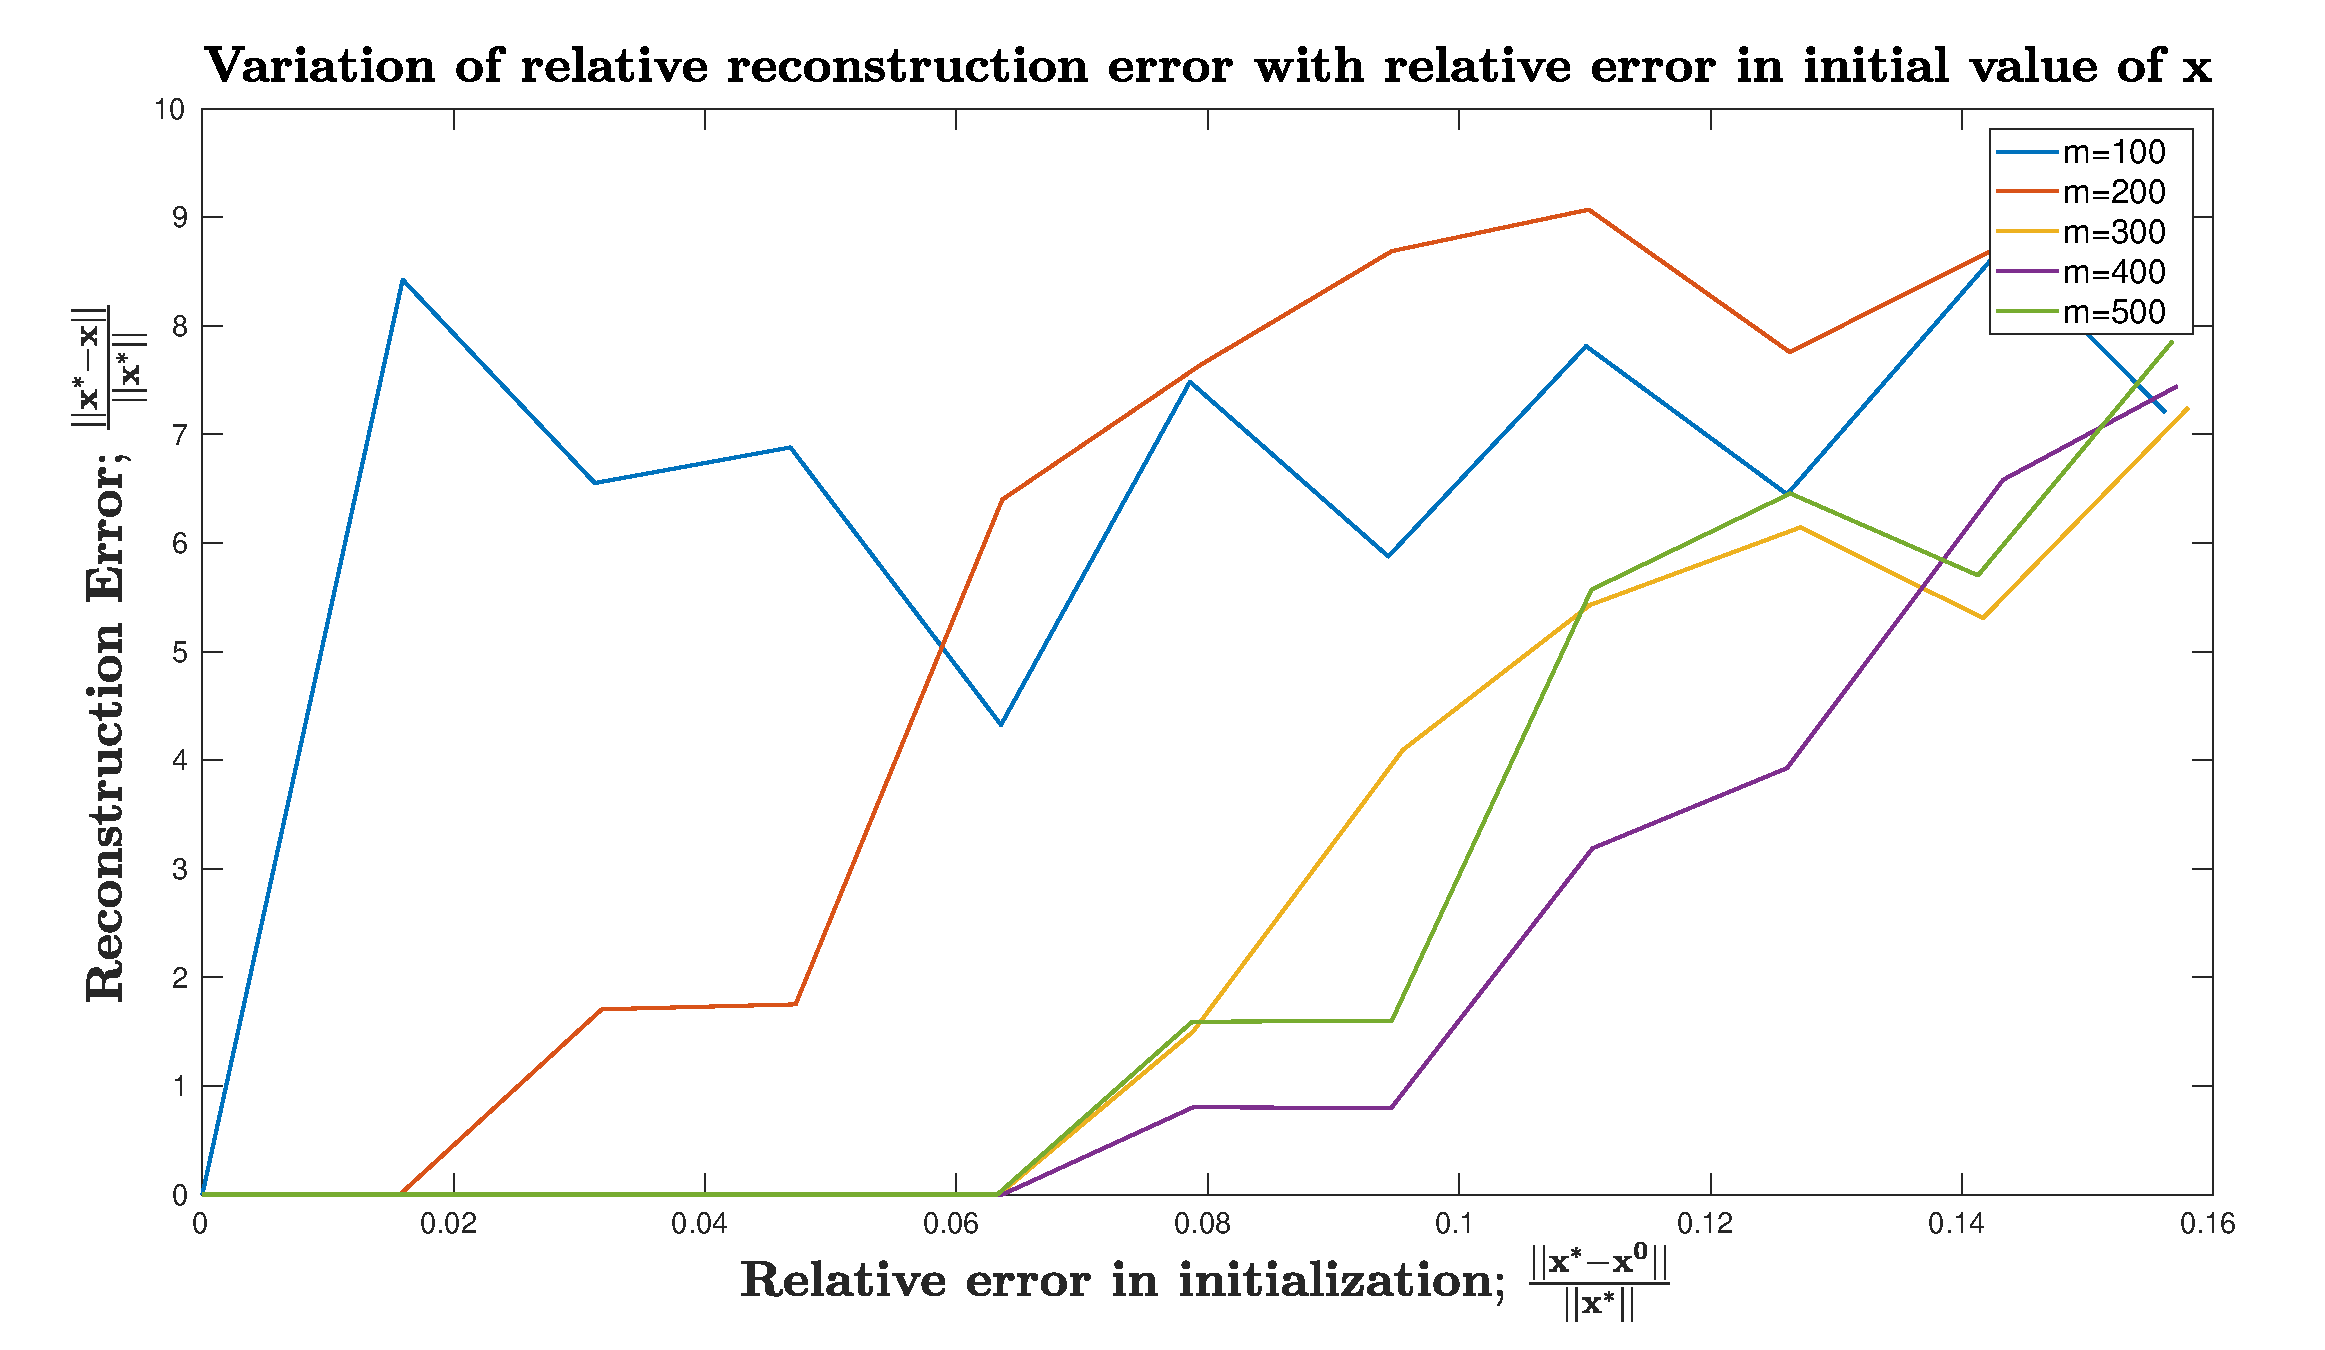
\includegraphics[width=\linewidth]{./fig/graph.pdf}
	\end{center}
	\caption{}
	\label{fig:pl}
\end{figure}

%\newpage
%\begin{section}{Appendix}
%\begin{figure}[t]
%	\begin{center}
%		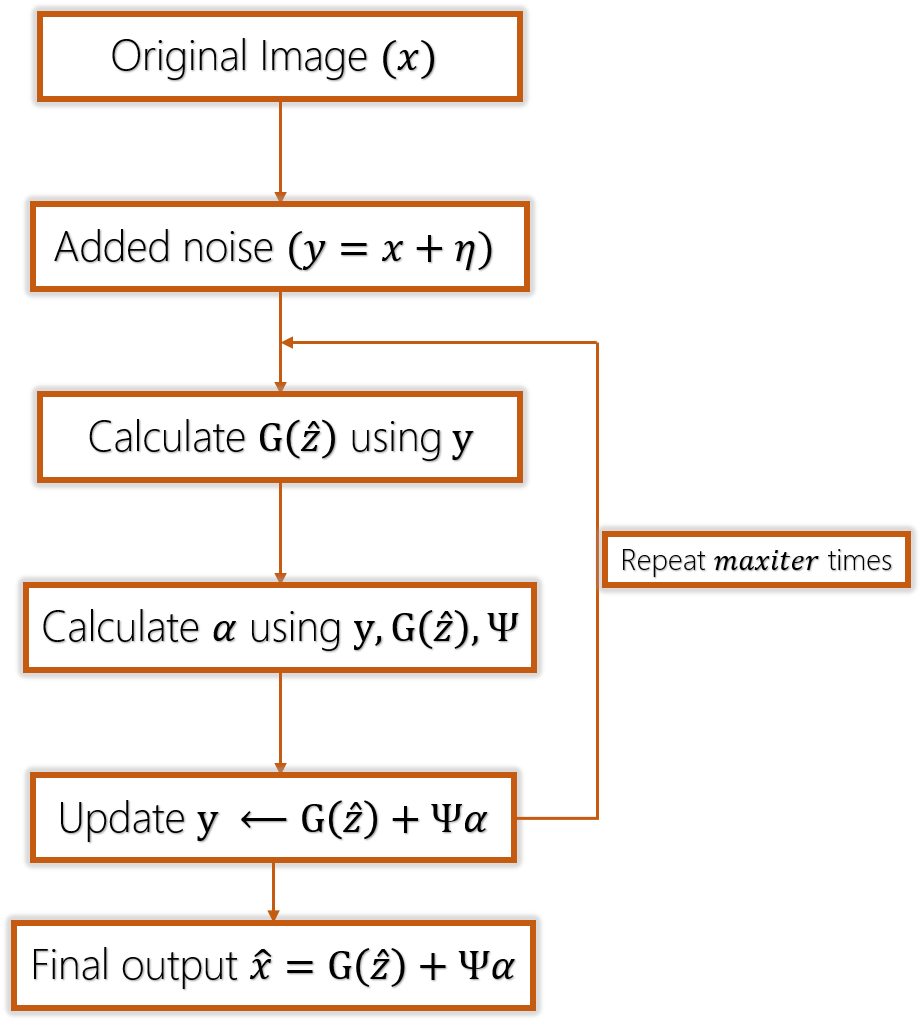
\includegraphics[width=0.4\linewidth]{./fig/alg.png}
%	\end{center}
%	\caption{\emph{Our approach}}
%	\label{fig:alg}
%\end{figure}
%\end{section}

\subsubsection{Performance of our algorithm for signal reconstruction}
We perform experiments on a synthetic signal generated randomly with $n=1000$ and $s=5$. We compute the initial estimate $\mathbf{x^0}$ using first order estimator method described in~\ref{sec:init}. we plot the variation of the relative reconstruction error ($\frac{\norm{\mathbf{x^*-x^N}}}{\norm{\mathbf{x^*}}}$) with number of measurements $m$ for both the variants of sparse recovery algorithm as described in~\ref{sec:altmin}.

It is important to note that unlike the absolute value function, the modulo function described in Fig.~\ref{fig:graph} is not scale-invariant. The modulo function works over the quantities $y_{c,i}=\langle \mathbf{a_i} \cdot \mathbf{x^*} \rangle, i=1,..,m$; and it is defined over the parameter $R$; thus depending on the magnitudes of $y_{c,i}$ and $R$ relative to each other, the behavior of the measurement model and the reconstruction algorithm would be altered. For instance, if the value of $R$ is too small compared to the range of the $y_{c,i}$, the modulo operation would hardly have any effect on the measurements, leaving $\mathbf{y_c \approx y}$. To analyze such variations, we fix the $R =1$ in our experiments, while varying the signal strength to vary the magnitudes of $y_{c,i}$. We measure the signal strength by the norm of the original signal ($\norm{\mathbf{{x}^*}}=1$).

Another important factor affecting the reconstruction is the quality of the initial estimate ($\mathbf{{x}^0}$) obtained through first order estimation. As described in~\ref{sec:init}, the quality of the initial estimate is a direct function of number of measurements ($m$). As we set $m$ higher, the initial estimate $\mathbf{{x}^0}$ would move closer to the original signal $\mathbf{{x}^*}$. For our experiments, we consider two ranges of $m$: $m \in [100,1000]$ and $m \in [1000,10000]$.
\begin{center}
	\begin{table}
		\centering
		\begin{tabular}{cccc}\toprule
			\multicolumn{4}{c}{\small{\textbf{Fixed:} $R=1, n=1000, s=5$}} \\ \midrule
			\multicolumn{2}{c}{\textbf{CoSaMP}}&\multicolumn{2}{c}{\textbf{robust CoSaMP}}
			\\\cmidrule(r){1-2}\cmidrule(r){3-4}  
			\small{$\norm{\mathbf{{x}^*}}=1$}&\small{$\norm{\mathbf{{x}^*}}=0.5$}&\small{$\norm{\mathbf{{x}^*}}=1$}&\small{$\norm{\mathbf{{x}^*}}=0.5$}\\\midrule
			\hyperref[fig:plot-1-1]{Figure~\ref{fig:plot-1-1}} & \hyperref[fig:plot-1-2]{Figure~\ref{fig:plot-1-2}}
			& \hyperref[fig:plot-1-3]{Figure~\ref{fig:plot-1-3}}  & \hyperref[fig:plot-1-4]{Figure~\ref{fig:plot-1-4}} \\
			\bottomrule
		\end{tabular}
		\caption{The Results}\label{Tab2}
	\end{table} 	
\end{center}


\begin{center}
	\begin{table}
		\centering
		\begin{tabular}{ccc}\toprule
			\multicolumn{3}{c}{\small{\textbf{Fixed:} $n=1000,\norm{\mathbf{{x}^*}}=1$}} \\ \midrule
			\multicolumn{3}{c}{\textbf{Justice Pursuit}}
			\\\cmidrule(r){1-3}%\cmidrule(r){3-4}  
			\small{$R =1$}&\small{$R=2$}&\small{$R=4$} \\\midrule
			\hyperref[fig:plot-2-1]{Figure~\ref{fig:plot-2-1}} & \hyperref[fig:plot-2-2]{Figure~\ref{fig:plot-2-2}}
			& \hyperref[fig:plot-2-3]{Figure~\ref{fig:plot-2-3}}   \\
			\bottomrule
		\end{tabular}
		\caption{The Results}\label{Tab3}
	\end{table} 	
\end{center}
In the Table~\ref{Tab2}, we provide experimental results for each of the combination above.

 
\begin{figure}[t]
	\begin{center}
		%\vspace{-0em}
		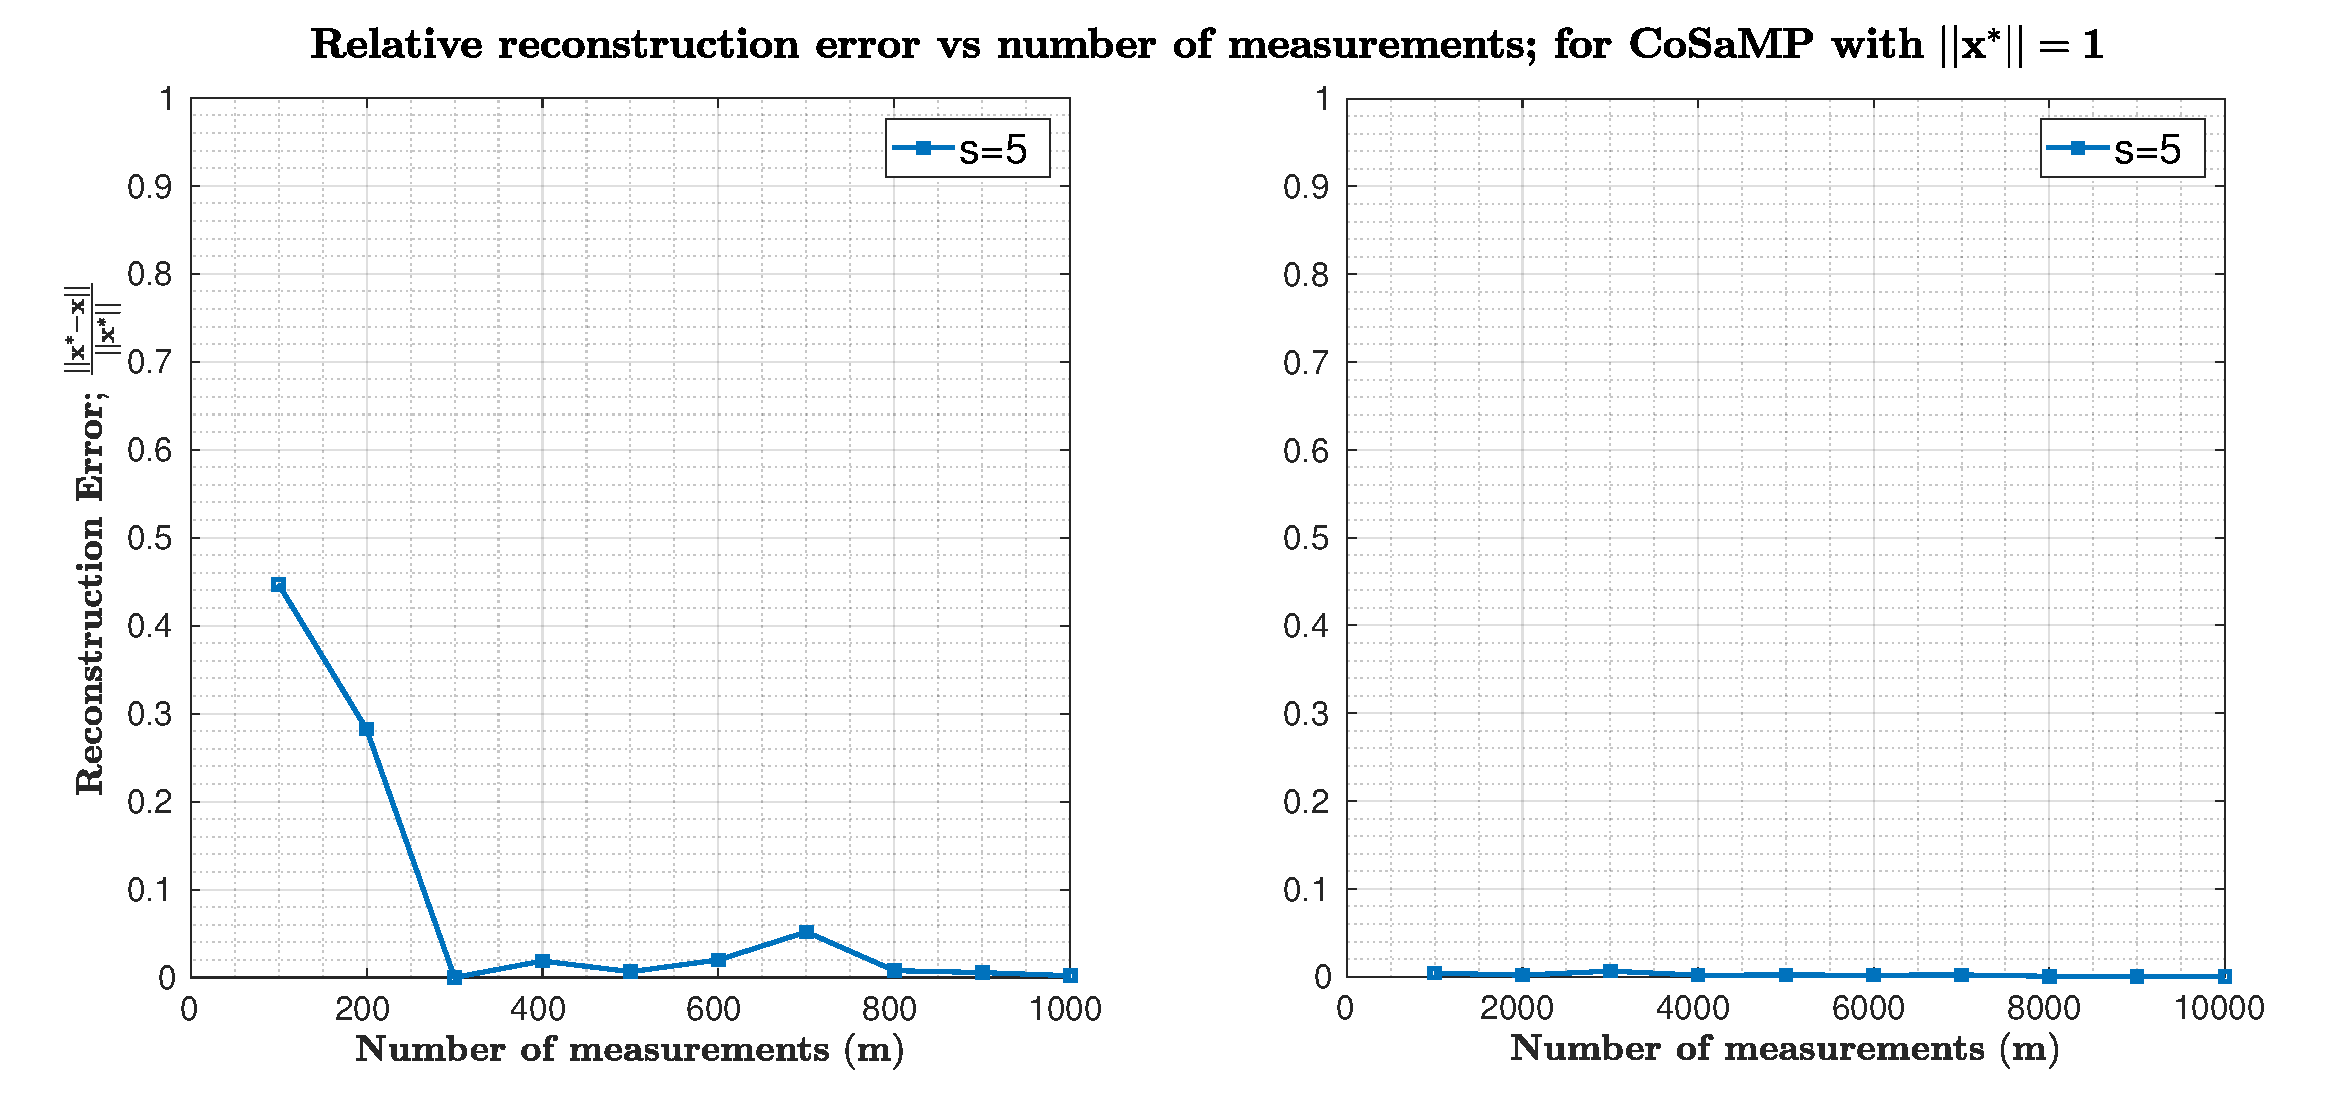
\includegraphics[width=\linewidth]{./fig/plot-1-1.pdf}
	\end{center}
	\caption{}
	\label{fig:plot-1-1}
\end{figure}

\begin{figure}[t]
	\begin{center}
		%\vspace{-0em}
		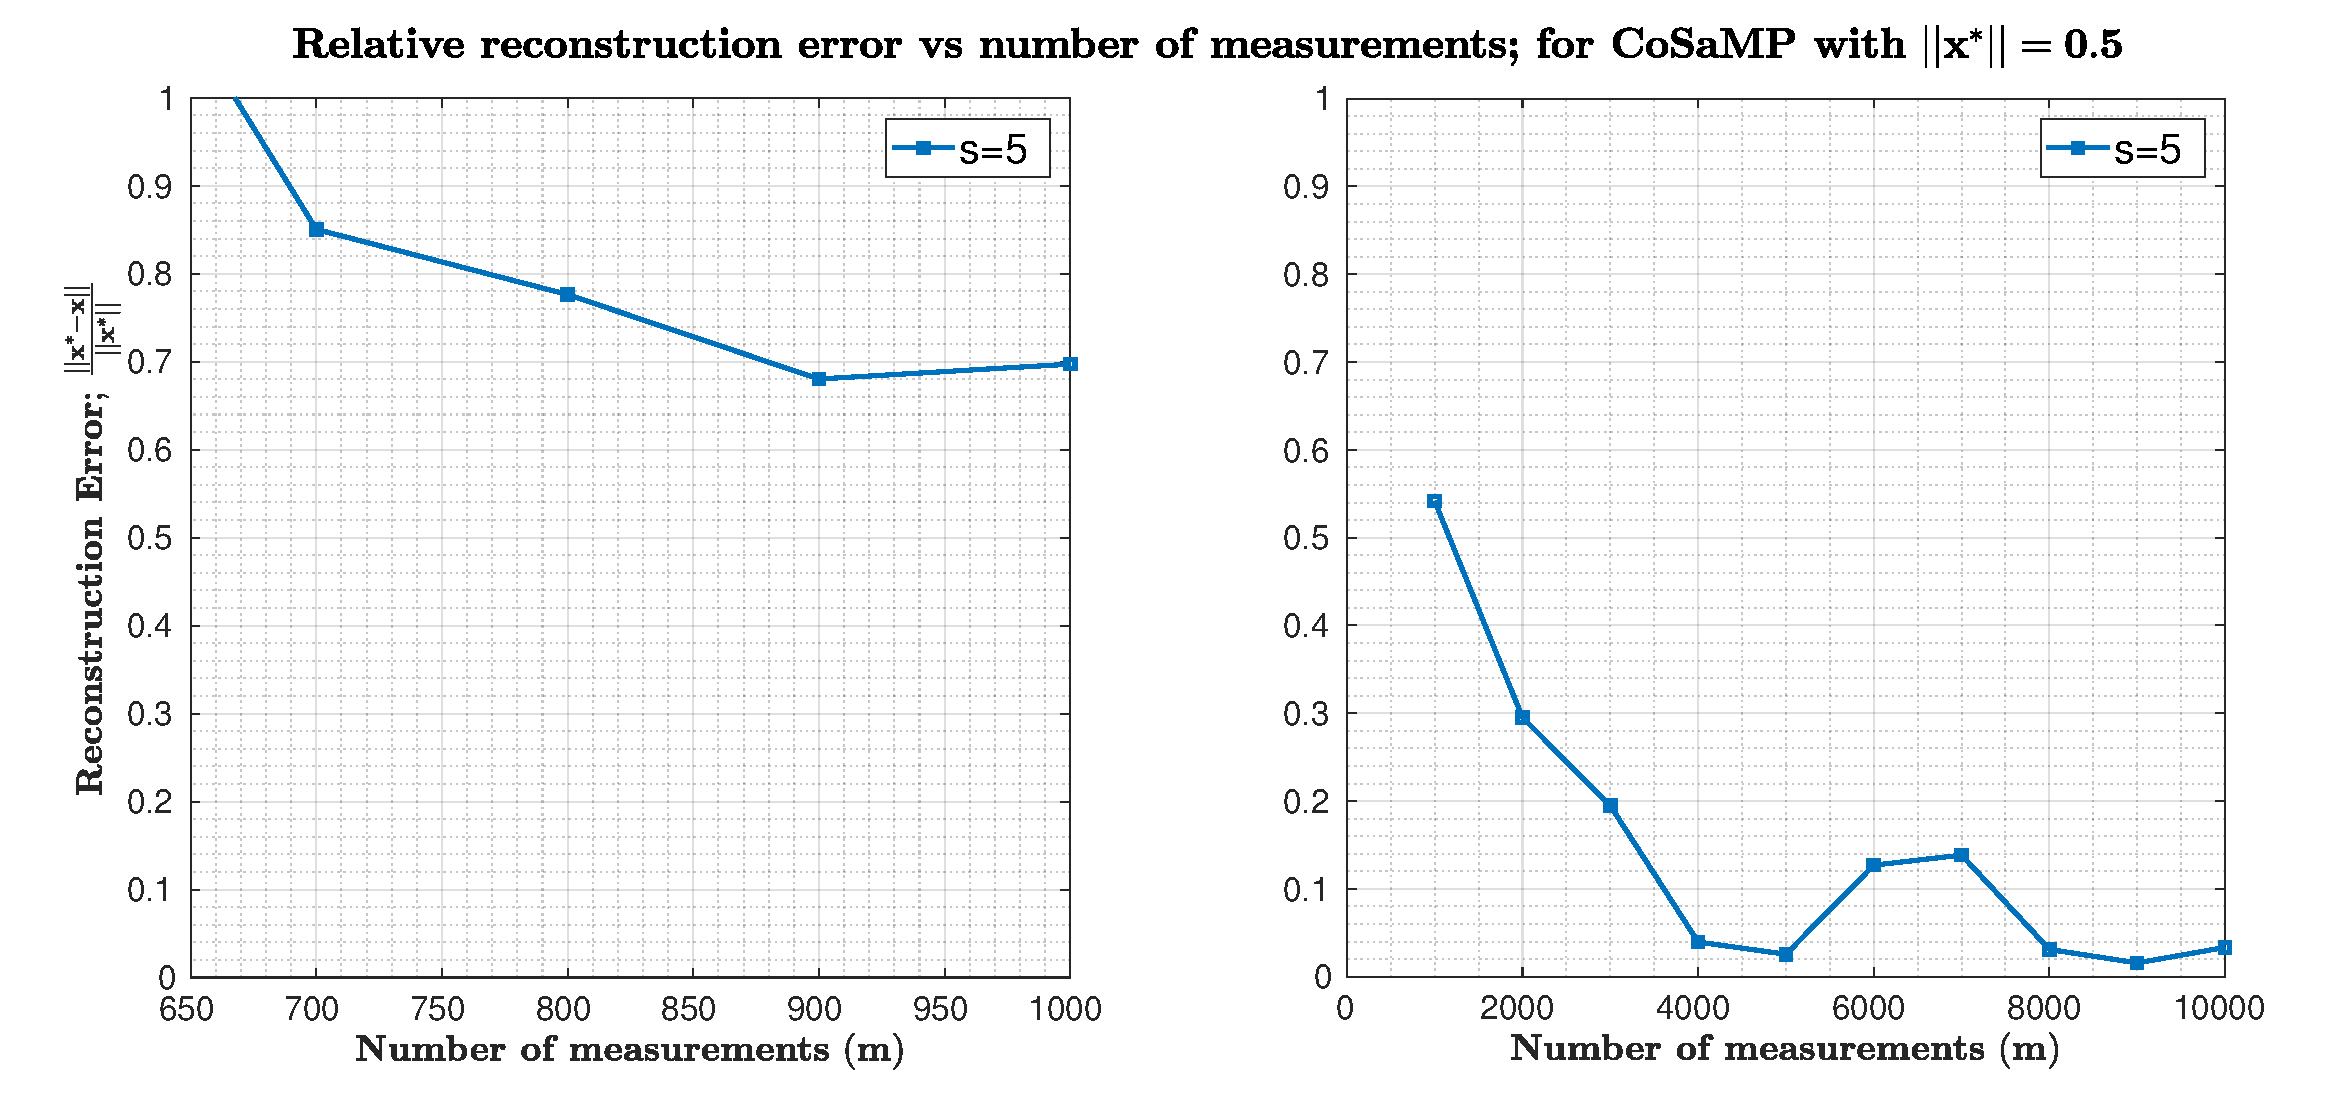
\includegraphics[width=\linewidth]{./fig/plot-1-2.pdf}
	\end{center}
	\caption{}
	\label{fig:plot-1-2}
\end{figure}
%
\begin{figure}[t]
	\begin{center}
		%\vspace{-0em}
		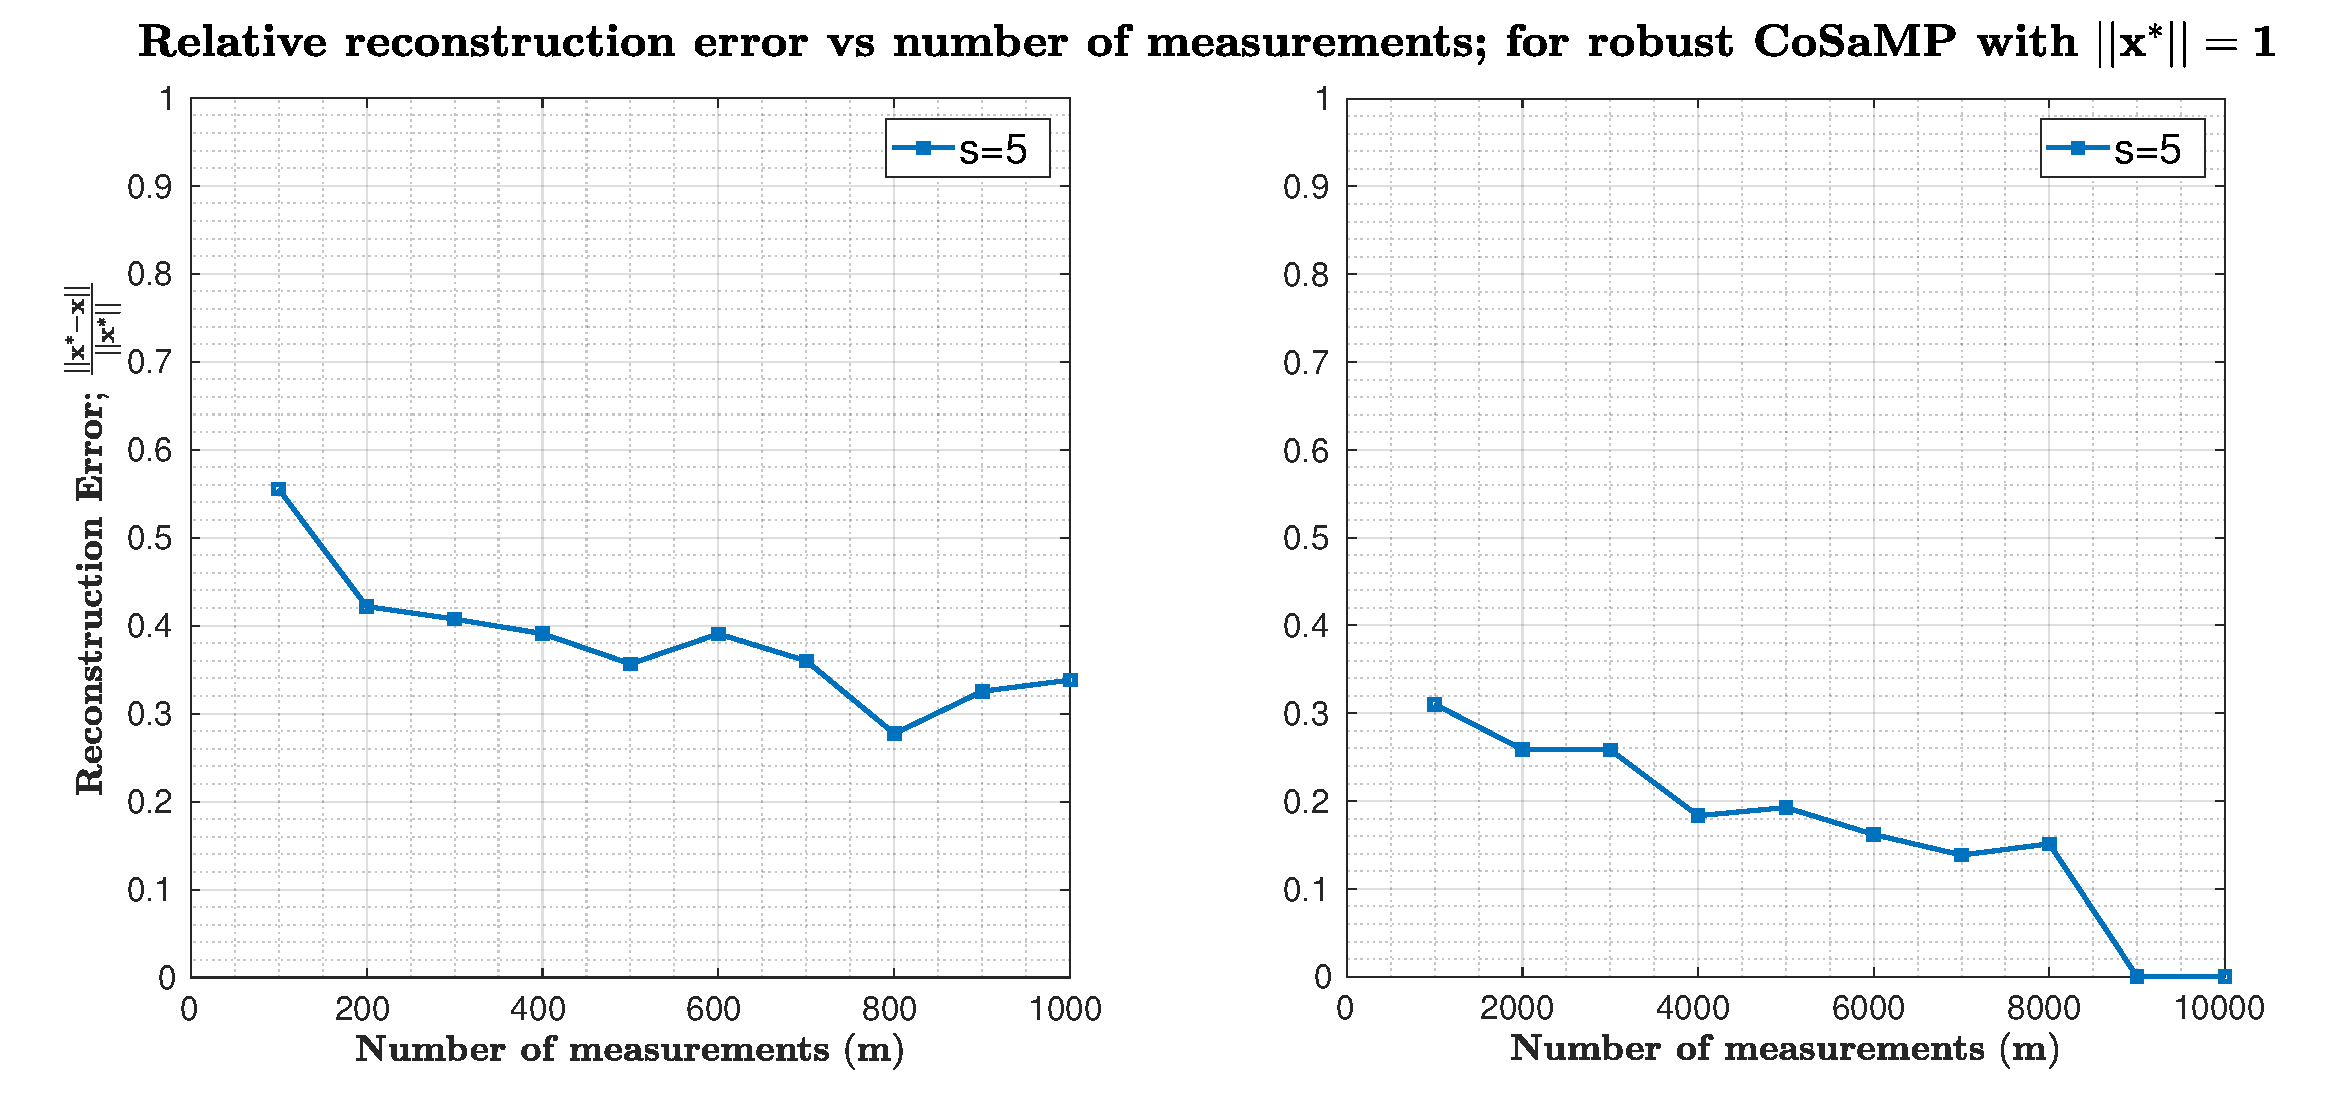
\includegraphics[width=\linewidth]{./fig/plot-1-3.pdf}
	\end{center}
	\caption{}
	\label{fig:plot-1-3}
\end{figure}
%
\begin{figure}[t]
	\begin{center}
		%\vspace{-0em}
		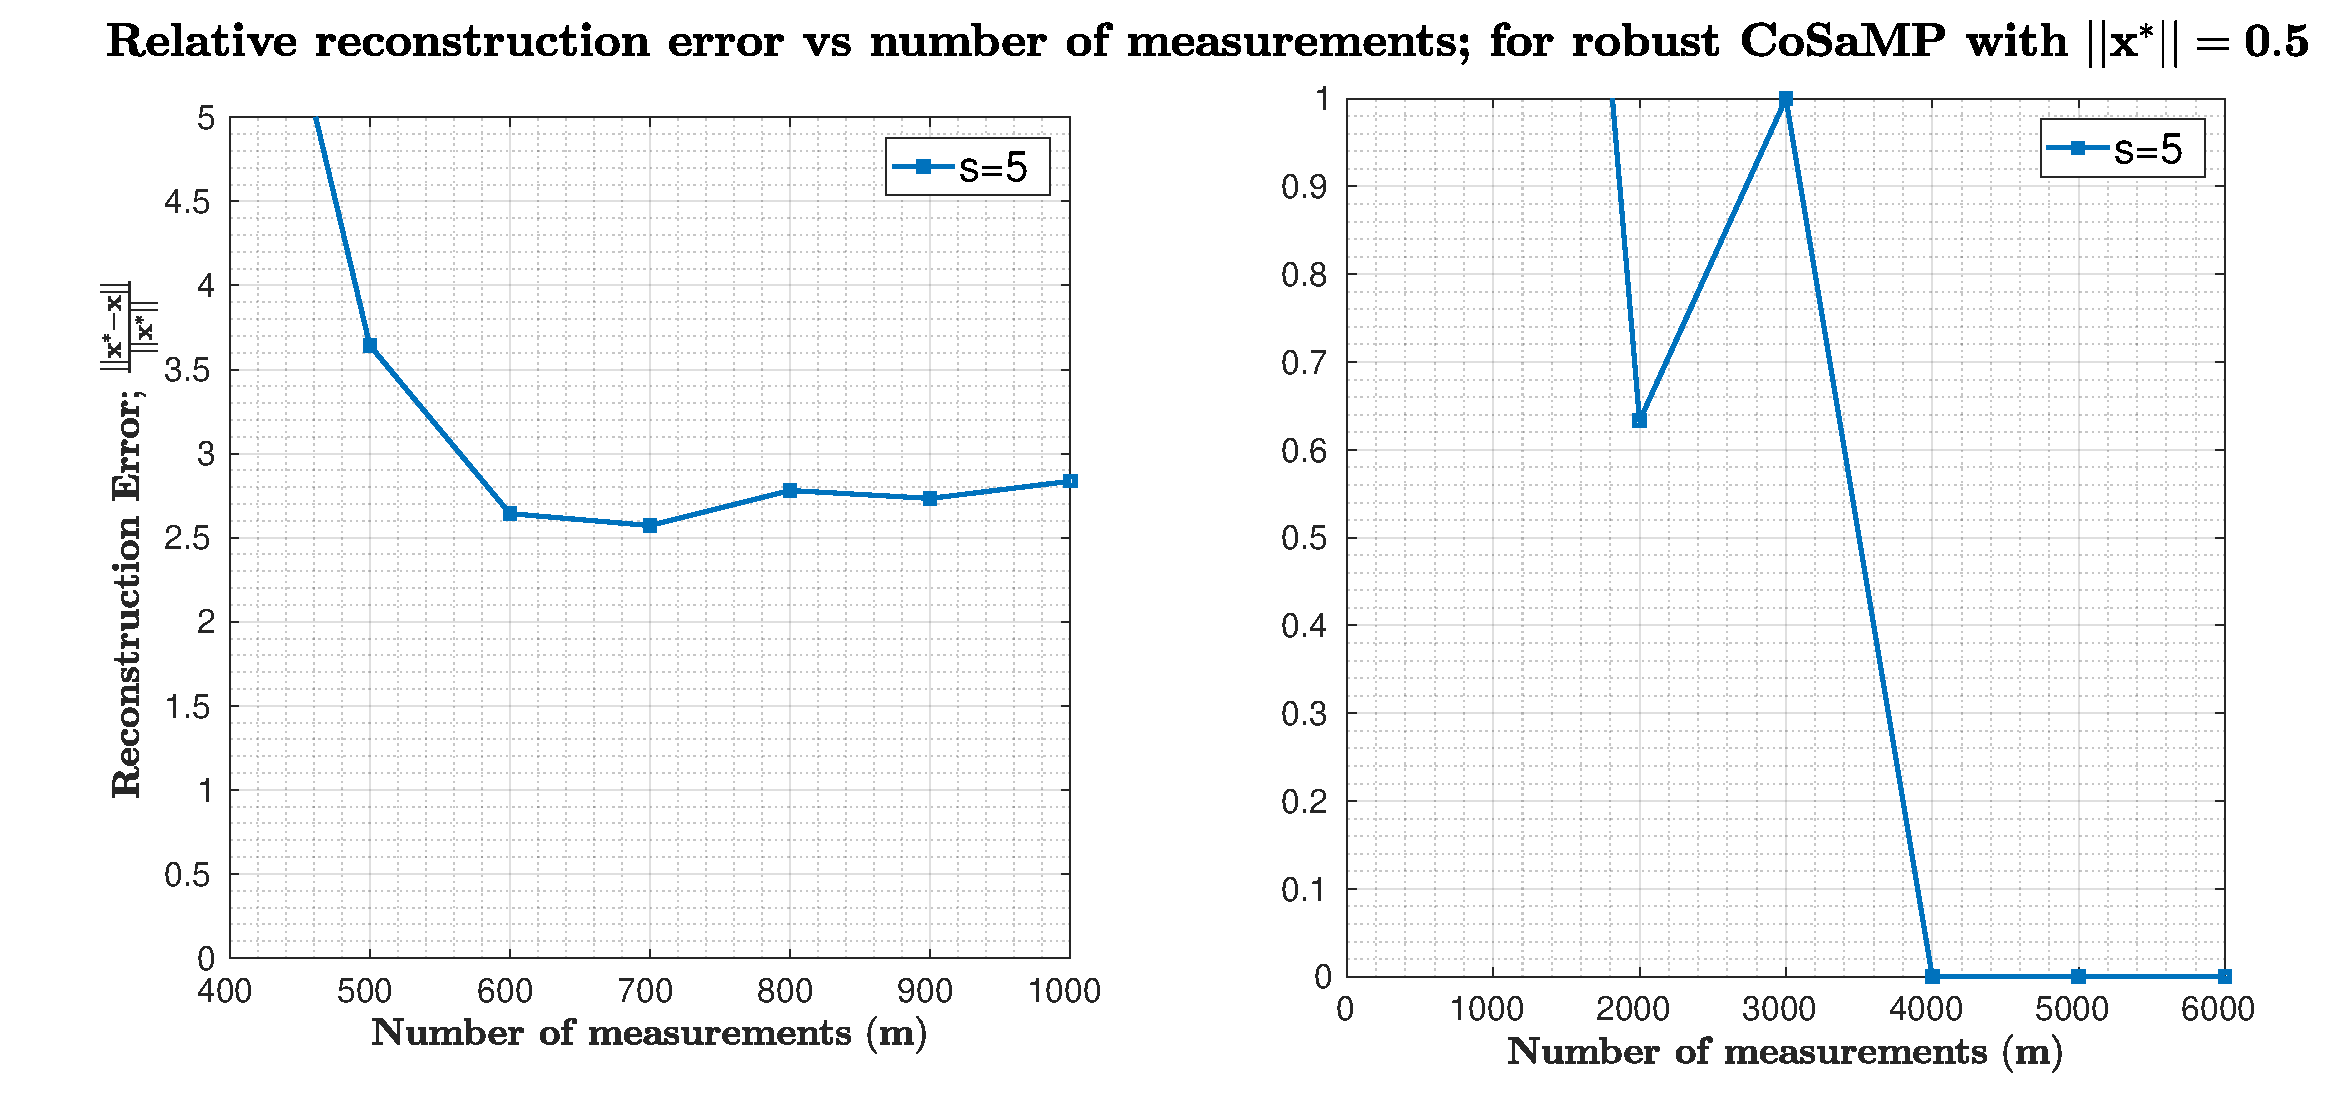
\includegraphics[width=\linewidth]{./fig/plot-1-4.pdf}
	\end{center}
	\caption{}
	\label{fig:plot-1-4}
\end{figure}






\begin{figure}[t]
	\begin{center}
		%\vspace{-0em}
		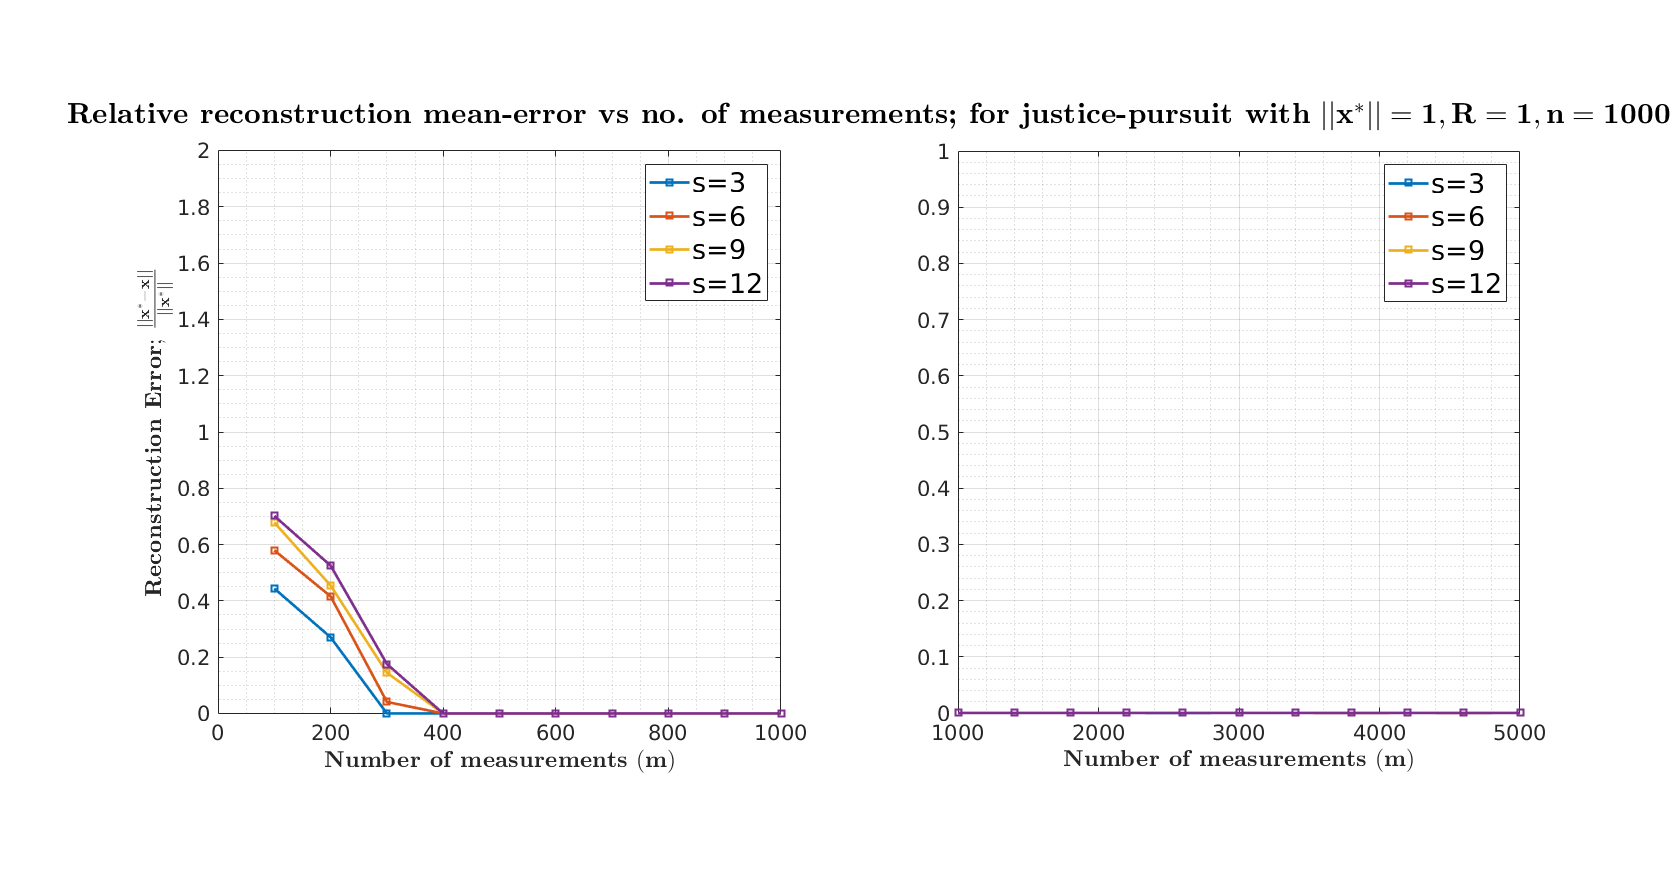
\includegraphics[width=\linewidth]{./fig/rcm_jp_r_1.png}
	\end{center}
	\caption{}
	\label{fig:plot-2-1}
\end{figure}


\begin{figure}[t]
	\begin{center}
		%\vspace{-0em}
		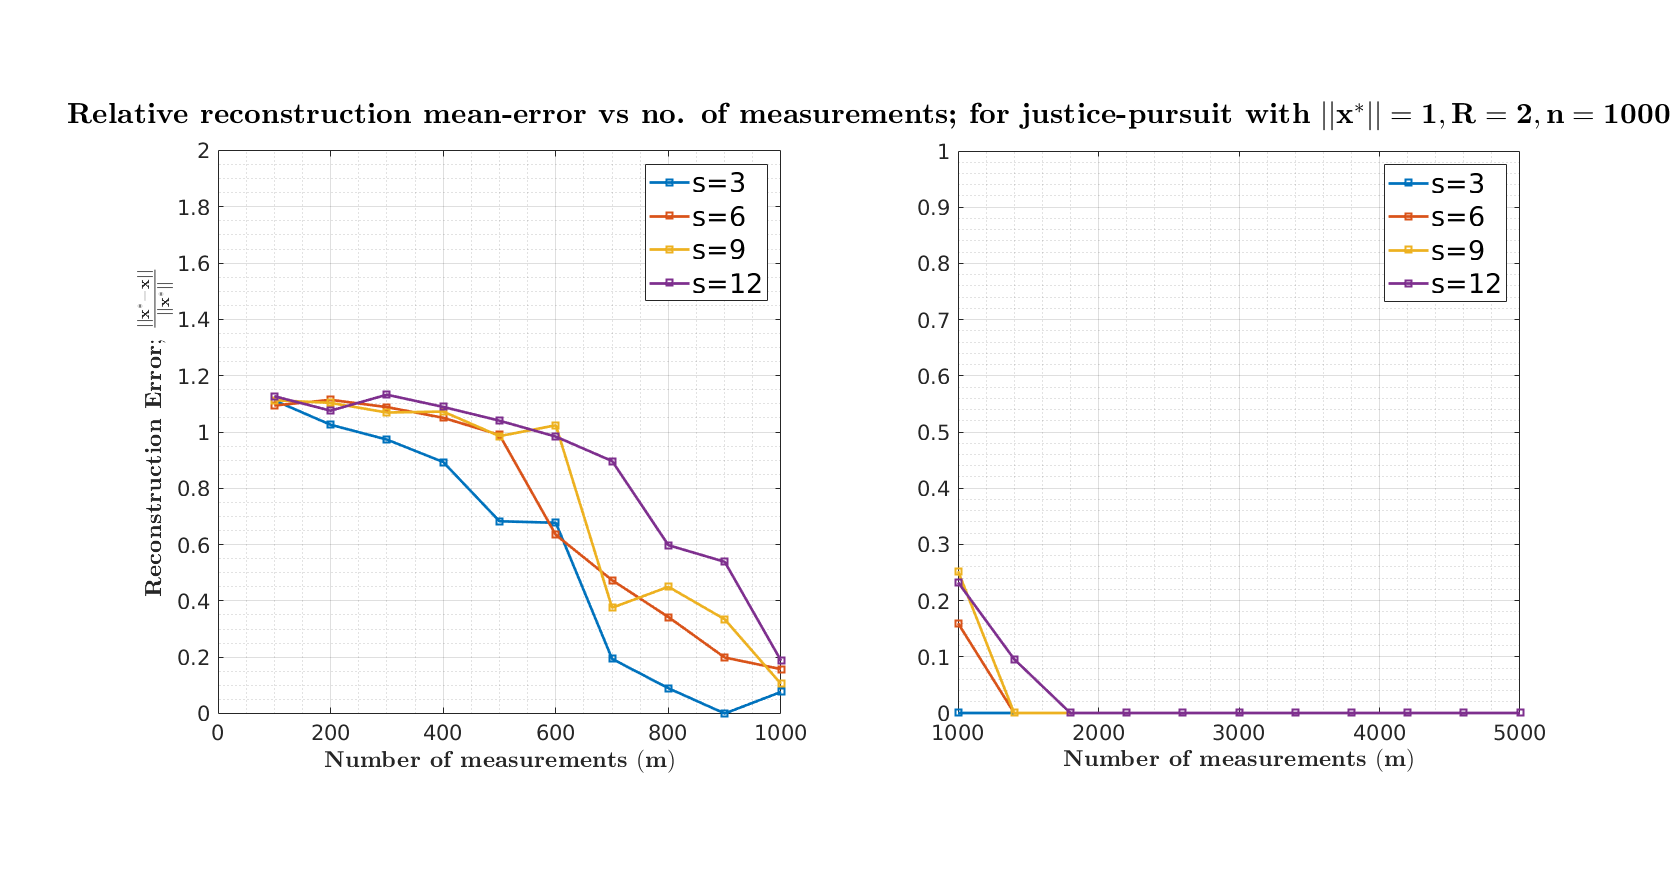
\includegraphics[width=\linewidth]{./fig/rcm_jp_r_2.png}
	\end{center}
	\caption{}
	\label{fig:plot-2-2}
\end{figure}


\begin{figure}[t]
	\begin{center}
		%\vspace{-0em}
		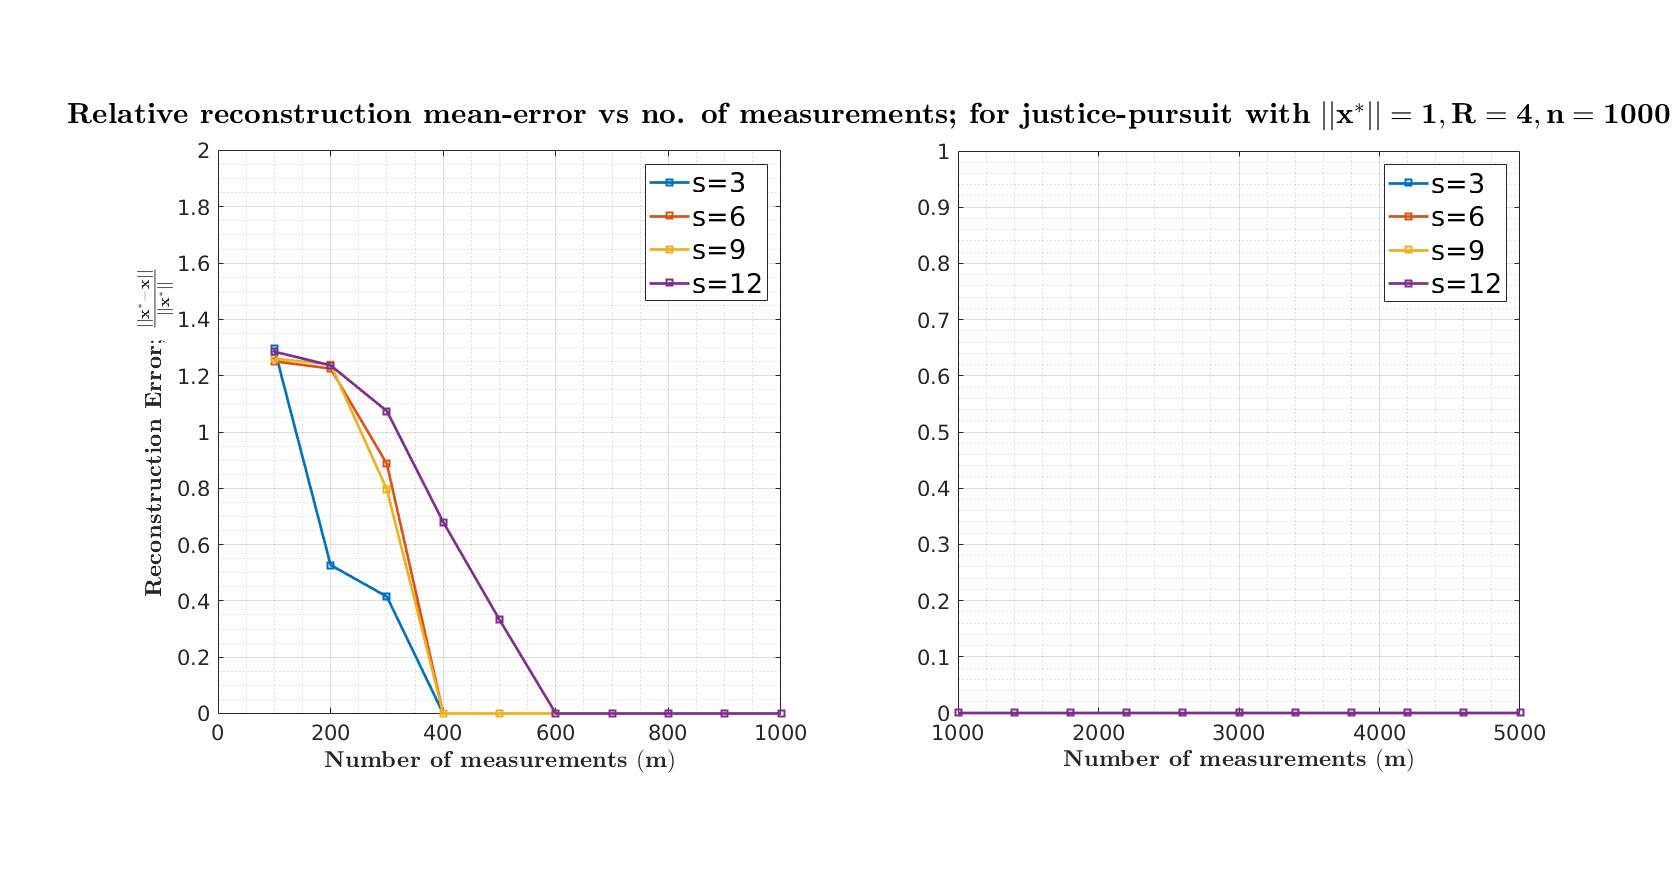
\includegraphics[width=\linewidth]{./fig/rcm_jp_r_4.png}
	\end{center}
	\caption{}
	\label{fig:plot-2-3}
\end{figure}